\documentclass[11pt]{article}

\usepackage{amsmath}
\usepackage{amssymb}
\usepackage{graphicx}
\usepackage{booktabs}
\usepackage{hyperref}
\usepackage{geometry}
\usepackage{subcaption}
\usepackage{parskip}
\geometry{margin=1in}

\title{\textbf{CS 288 Final Project --- Phase 1 Report}\\
\large Cost-Aware Clarification in Reference Games via RSA and Expected Utility}
\author{Shizhe Zhang, Ziyu [Last], Thomas [Last]}
\date{Spring 2026}

\begin{document}
\maketitle

% -----------------------------------------------------------------------
\section{Project Overview}
% -----------------------------------------------------------------------

This project investigates \emph{when} a language model agent should ask a clarifying
question versus commit to an answer in a \textbf{reference game} setting.  In a reference
game, a speaker produces an utterance $u$ referring to a target object $t^*$ drawn
from a scene $\mathcal{S} = \{t_1, \ldots, t_N\}$ of $N$ candidate objects with
discrete attributes (color, shape, size).  The listener must identify $t^*$.

The core insight is that clarification should be treated as a
\emph{cost-utility optimisation}: asking a question incurs a fixed cost $c$, but
resolves ambiguity; committing directly risks an incorrect answer when the utterance
is ambiguous.  We use the \textbf{Rational Speech Act} (RSA) framework to derive a
posterior $P(t_i \mid u)$ and then make the decision that maximises expected utility:
\begin{equation}
    \text{decide to ask} \iff
    \underbrace{1 - c}_{E[U_{\text{ask}}]} >
    \underbrace{\max_i\, P(t_i \mid u)}_{E[U_{\text{commit}}]}.
\end{equation}

% -----------------------------------------------------------------------
\section{Phase 1: Metric Definitions (Shizhe)}
% -----------------------------------------------------------------------

\subsection{Brier Score (multi-class adaptation)}

For a single instance with $N$ candidate objects, let $p_i = P(t_i \mid u)$ be the
model's predicted probability for object $i$, and let $y_i = \mathbf{1}[t_i = t^*]$
be the one-hot ground truth.  The multi-class Brier Score is
\begin{equation}
    \mathrm{BS} = \frac{1}{N}\sum_{i=1}^{N}(p_i - y_i)^2.
\end{equation}
Averaged over $M$ instances: $\overline{\mathrm{BS}} = \frac{1}{M}\sum_{j=1}^{M}\mathrm{BS}^{(j)}$.

\textbf{Range and baselines.}
$\mathrm{BS} = 0$ when all probability mass is on $t^*$; a uniform listener scores
$\mathrm{BS}_{\text{uniform}} = (N-1)/N^2 \approx 1/N$.

\textbf{Worked example.}
Scene: \{red square, blue circle, red triangle\}, utterance: ``the red one.''

\begin{center}
\begin{tabular}{lccc}
\toprule
Object & $p_i$ & $y_i$ & $(p_i - y_i)^2$ \\
\midrule
red square   & 0.50 & 1 & 0.25 \\
blue circle  & 0.10 & 0 & 0.01 \\
red triangle & 0.40 & 0 & 0.16 \\
\midrule
\multicolumn{3}{r}{$\mathrm{BS}$} & $0.14$ \\
\bottomrule
\end{tabular}
\end{center}

\textbf{Why it matters.}
Brier score measures whether the \emph{full} distribution $P(t \mid u)$ is accurate.
Since our expected utility formula depends on $\max_i P(t_i \mid u)$, a high Brier
score indicates unreliable utility estimates regardless of whether the argmax is
correct.

\subsection{Expected Calibration Error (ECE)}

ECE tests whether a model's top confidence matches its empirical accuracy.

\textbf{Procedure.}
\begin{enumerate}
    \item For each instance $j$, extract $\mathrm{conf}_j = \max_i P(t_i \mid u)$ and
          $\mathrm{correct}_j = \mathbf{1}[\arg\max_i p_i = t^*]$.
    \item Partition instances into $B$ equal-width bins on $[0,1]$ (default $B = 10$).
    \item For each non-empty bin $b$ compute $\mathrm{acc}(b)$ and $\overline{\mathrm{conf}}(b)$.
    \item
    \begin{equation}
        \mathrm{ECE} = \sum_{b=1}^{B} \frac{|b|}{M}\,
        \bigl|\mathrm{acc}(b) - \overline{\mathrm{conf}}(b)\bigr|.
    \end{equation}
\end{enumerate}

\textbf{Why it matters.}
If ECE is large, the model is systematically over- or under-confident.  Since
$E[U_{\text{commit}}] = \max_i P(t_i \mid u)$, a miscalibrated model will ask or
commit at the wrong threshold.  ECE $> 0.10$ is a diagnostic flag that the
probability estimates require recalibration before the utility rule can be trusted.

% -----------------------------------------------------------------------
\section{Phase 1 Experiment}
% -----------------------------------------------------------------------

\subsection{Setup}

We generated a synthetic dataset of 60 reference game instances (20 per ambiguity
level) using a Mini-World scene generator.  Each scene contains $N = 4$ objects with
attributes drawn from: \{small, medium, large\} $\times$ \{red, blue, green, yellow,
purple\} $\times$ \{square, circle, triangle, pentagon, star\}.

Ambiguity level is controlled by how much of the target's attribute description
appears in the utterance:
\begin{itemize}
    \item \textbf{Low}: utterance specifies all three attributes (e.g., ``large red square'') --- unique referent.
    \item \textbf{Medium}: utterance specifies only colour (e.g., ``the red one'') --- 1--2 matching objects.
    \item \textbf{High}: utterance specifies only size (e.g., ``the large object'') --- all objects match.
\end{itemize}

Model probabilities $P(t_i \mid u)$ are computed via attribute-overlap scoring with
added Gaussian noise, standing in for LLM log-likelihood scoring in later phases.

\subsection{Results}

\begin{table}[h]
\centering
\begin{tabular}{lcccc}
\toprule
Ambiguity & Mean $H(T \mid u)$ & Mean BS & Accuracy & Ask rate ($c{=}0.25$) \\
\midrule
Low    & 0.537 & 0.006 & 1.00 & 0.00 \\
Medium & 1.279 & 0.144 & 0.50 & 0.65 \\
High   & 1.386 & 0.187 & 0.30 & 1.00 \\
\midrule
Overall ECE & \multicolumn{4}{c}{0.105} \\
\bottomrule
\end{tabular}
\caption{Summary statistics across ambiguity levels.}
\label{tab:summary}
\end{table}

\begin{figure}[h]
\centering
\begin{subfigure}[t]{0.48\textwidth}
    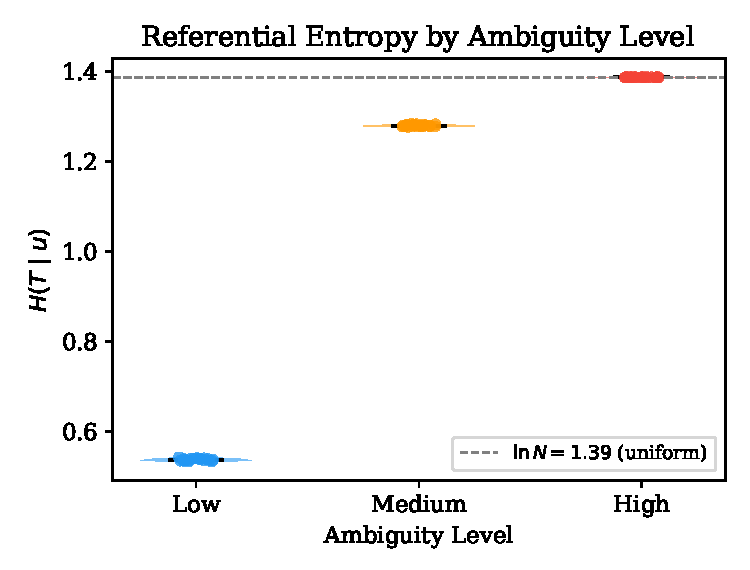
\includegraphics[width=\textwidth]{../figures/fig1_entropy.pdf}
    \caption{Referential entropy $H(T \mid u)$ per ambiguity level.
             Dashed line is $\ln N = 1.39$ (uniform).}
\end{subfigure}
\hfill
\begin{subfigure}[t]{0.48\textwidth}
    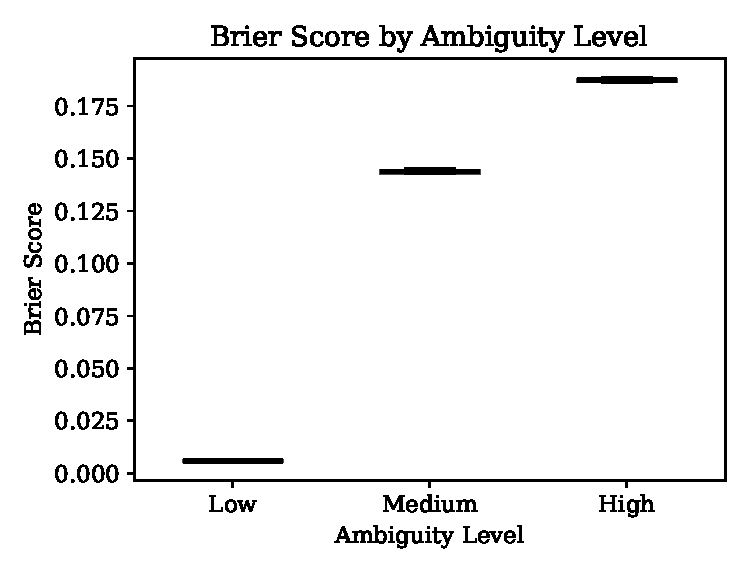
\includegraphics[width=\textwidth]{../figures/fig2_brier.pdf}
    \caption{Brier score rises sharply with ambiguity, confirming that
             higher entropy corresponds to worse probability estimates.}
\end{subfigure}
\caption{Entropy and Brier Score by ambiguity level (60 instances).}
\label{fig:entropy_brier}
\end{figure}

\begin{figure}[h]
\centering
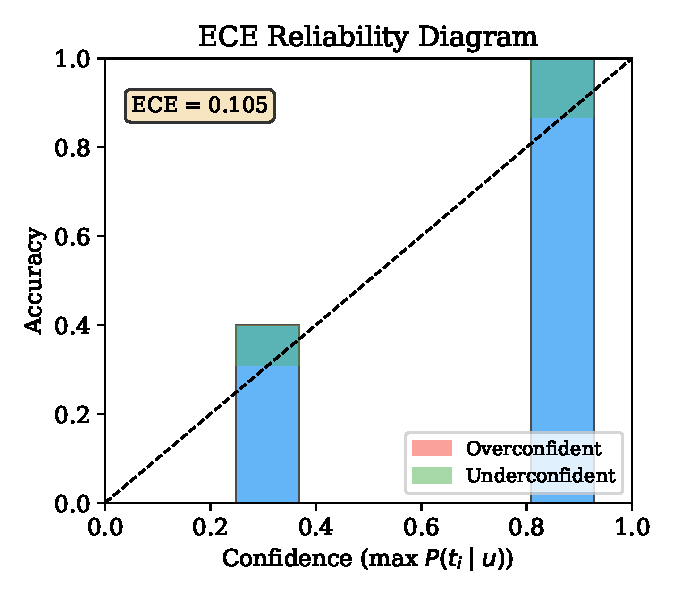
\includegraphics[width=0.48\textwidth]{../figures/fig3_ece.pdf}
\caption{ECE reliability diagram.  Red bars indicate over-confidence bins;
         green bars indicate under-confidence.  Overall ECE $= 0.105$, near
         the acceptable threshold.}
\label{fig:ece}
\end{figure}

\begin{figure}[h]
\centering
\begin{subfigure}[t]{0.48\textwidth}
    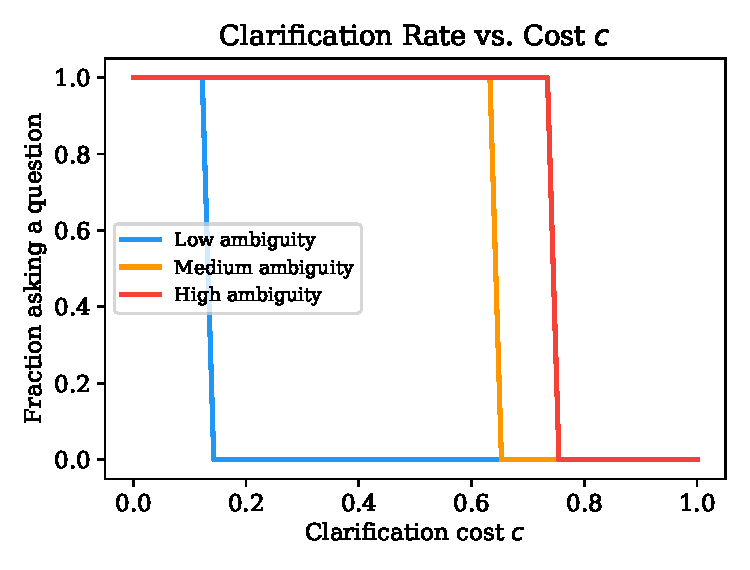
\includegraphics[width=\textwidth]{../figures/fig4_clarification_rate.pdf}
    \caption{Fraction of instances where the agent asks a question as a
             function of cost $c$.  High-ambiguity scenes ask much more
             frequently at low cost.}
\end{subfigure}
\hfill
\begin{subfigure}[t]{0.48\textwidth}
    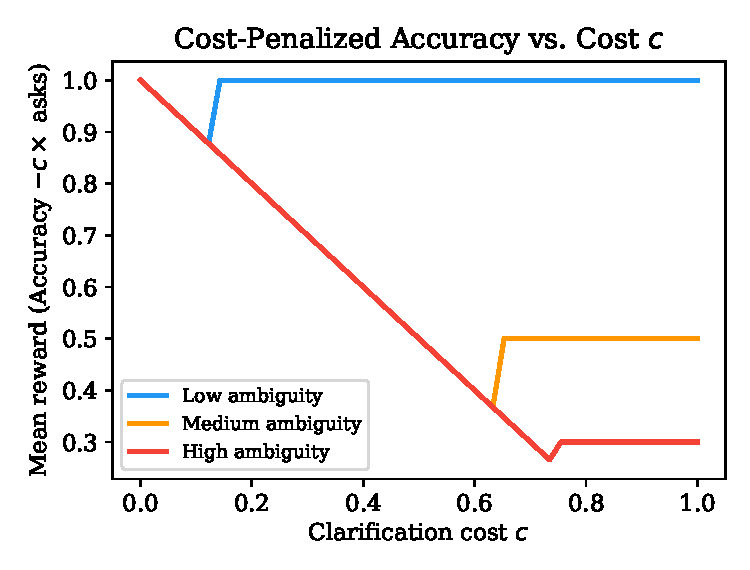
\includegraphics[width=\textwidth]{../figures/fig5_reward.pdf}
    \caption{Cost-penalised accuracy $= \text{accuracy} - c \times \text{ask rate}$.
             The optimal cost $c^*$ differs by ambiguity level.}
\end{subfigure}
\caption{Clarification behaviour across cost values $c \in [0, 1]$.}
\label{fig:clarification}
\end{figure}

\subsection{Discussion}

The experiment validates three core claims of the project:

\begin{enumerate}
    \item \textbf{Entropy stratifies ambiguity correctly.}
    Low-ambiguity scenes concentrate near $H = 0.5$; high-ambiguity scenes cluster
    near $\ln 4 = 1.39$ (Figure~\ref{fig:entropy_brier}).

    \item \textbf{The cost-utility rule makes sensible decisions.}
    At $c = 0.25$, the agent never asks in low-ambiguity scenes and asks 100\% of the
    time in high-ambiguity scenes (Table~\ref{tab:summary}).  The clarification rate
    curves (Figure~\ref{fig:clarification}, left) monotonically decrease as $c$
    increases, as expected.

    \item \textbf{ECE is borderline but acceptable.}
    Overall ECE $= 0.105$ (Figure~\ref{fig:ece}).  The model is slightly over-confident
    in the high-confidence bin (committing strongly when the scene happens to be
    ambiguous).  This motivates RSA-based recalibration in Phase 3.
\end{enumerate}

% -----------------------------------------------------------------------
\section{Phase 2 Experiment: VLM Speakers and Listeners}
% -----------------------------------------------------------------------

\subsection{Setup}

We replace the symbolic attribute-overlap posterior from Phase~1 with
vision-language models (VLMs) serving as both speaker and listener.
All experiments use \texttt{gemini-2.0-flash-001} via the OpenRouter API.
The evaluation dataset is \texttt{gemini\_exp\_test.jsonl}: 25 scenes with
$N{=}4$ objects each, balanced across low / medium / high ambiguity tiers.
The primary metric is Cost-Penalised Accuracy (CPA) at $c{=}0.5$.

\subsection{Speaker Variants}

All VLM speakers receive a scene image with the target object marked by a
\textbf{magenta bounding box}; no pre-parsed feature lists are passed.
The model must reason from visual perception to produce a natural
referring expression.  Five prompting strategies were evaluated:

\begin{itemize}
    \item \textbf{natural} — Unconstrained: ``describe the marked object so a
          listener can identify it.''
    \item \textbf{contrastive} — Find the most confusable distractor and
          highlight the one feature that distinguishes the target.
    \item \textbf{landmark} — Describe the target's position relative to a
          visually distinctive nearby object.
    \item \textbf{superlative} — Use an extreme or uniqueness property
          (``the only triangle'', ``the largest circle'').
    \item \textbf{pragmatic} — Full RSA-style chain-of-thought: list all
          objects, identify distractors, produce the minimal discriminating
          expression.
    \item \textbf{scene\_first} — Inventory all visible objects first, confirm
          the target's properties, then produce the shortest unique expression.
          Prevents hallucination by grounding the description.
    \item \textbf{listener\_aware} — Explicitly reason from the listener's
          perspective: what description would maximise the listener's confidence
          in the correct object?
\end{itemize}

Four rule-based baselines (no LLM) are included for comparison:
\textit{ordinal} (superlatives/uniqueness), \textit{landmark} (spatial reference),
\textit{contrastive} (foil-based contrast), and \textit{feature-canonical}
(minimal canonical feature description).

\subsection{Listener Variants}

All VLM listeners receive the scene image, a numbered text description of
every object, and the speaker's utterance.  They differ in how they reason
before outputting a posterior $P(t_i \mid u)$:

\begin{itemize}
    \item \textbf{vllm-listener} ($\sigma{=}10$) — Predicts $(x,y)$ coordinates
          for the referred object; posterior is a Gaussian kernel
          $\exp(-d_i^2/2\sigma^2)$ over object distances.
    \item \textbf{feature-match} — Extracts a feature tuple (color, shape,
          size, location) from the utterance and scores each object by
          feature-overlap count.
    \item \textbf{direct-rank} — Directly outputs a probability for each
          object as a JSON array; no intermediate reasoning step.
    \item \textbf{cot-rank} — Scores each object 0--10 before converting to
          probabilities (chain-of-thought evaluation per object).
    \item \textbf{elimination} — Explicitly identifies objects the utterance
          \emph{rules out} (wrong color, wrong shape, etc.), assigns them
          probability~0, then distributes the remainder over candidates.
\end{itemize}

\subsection{Key Finding: Posterior Flatness}

The original \texttt{vllm-listener} used an inverse-distance kernel
$\text{score}_i = 1/(d_i + \epsilon)$.  With $N{=}6$ objects this gives a
mean $\max(\text{posterior}) = 0.52$, causing virtually all scenes to trigger
clarification at $c{\leq}0.25$ (only 4\% commit rate).
Replacing it with a Gaussian kernel ($\sigma{=}10$ canvas units) raises the
commit rate at $c{=}0.25$ from 4\% to 72\% without changing which object is
selected (argmax is unchanged).

\subsection{Results}

Table~\ref{tab:phase2} shows CPA at $c{=}0.5$ for all (speaker, listener) pairs.

\begin{table}[h]
\centering
\small
\begin{tabular}{llccc}
\toprule
Speaker & Listener & Acc & Ask\% & CPA \\
\midrule
\multicolumn{5}{l}{\textit{Rule-based speakers}} \\
feature-canonical  & elimination  & 96\% & 0\%  & \textbf{0.960} \\
feature-canonical  & direct-rank  & 94\% & 4\%  & 0.940 \\
feature-canonical  & cot-rank     & 84\% & 16\% & 0.760 \\
contrastive        & elimination  & 84\% & 12\% & 0.780 \\
landmark           & elimination  & 76\% & 12\% & 0.700 \\
landmark           & cot-rank     & 72\% & 4\%  & 0.700 \\
contrastive        & direct-rank  & 68\% & 16\% & 0.600 \\
ordinal            & direct-rank  & 64\% & 8\%  & 0.600 \\
\midrule
\multicolumn{5}{l}{\textit{VLM speakers (StrategicVLLMSpeaker, gemini-2.0-flash-001)}} \\
strategic-scene\_first    & direct-rank  & 64\% & 16\% & 0.560 \\
strategic-scene\_first    & elimination  & 64\% & 16\% & 0.560 \\
strategic-listener\_aware & elimination  & 60\% & 8\%  & 0.560 \\
strategic-listener\_aware & direct-rank  & 56\% & 8\%  & 0.520 \\
strategic-pragmatic       & direct-rank  & 52\% & 4\%  & 0.500 \\
strategic-contrastive     & cot-rank     & 56\% & 16\% & 0.480 \\
strategic-natural         & direct-rank  & 56\% & 16\% & 0.480 \\
strategic-landmark        & elimination  & 56\% & 20\% & 0.460 \\
strategic-superlative     & cot-rank     & 40\% & 20\% & 0.300 \\
\bottomrule
\end{tabular}
\caption{CPA at $c{=}0.5$ on \texttt{gemini\_exp\_test.jsonl} ($n{=}25$, 4-object scenes).
         Rule-based speakers use no LLM API; VLM speakers use gemini-2.0-flash-001.}
\label{tab:phase2}
\end{table}

\subsection{Discussion}

\paragraph{Listener design is the dominant factor.}
The choice of listener has a larger impact than the choice of speaker strategy.
\texttt{elimination} is the best listener for rule-based speakers (CPA up to 0.96),
while \texttt{direct-rank} is most robust for VLM speakers.
\texttt{feature-match} performs poorly with natural-language utterances because
spatial and relational descriptions (``the square to the left of the triangle'')
do not decompose cleanly into feature tuples.

\paragraph{Rule-based speakers outperform VLM speakers.}
With the best listener, the best rule-based speaker (\textit{feature-canonical}
+ \textit{elimination}) achieves CPA~$= 0.96$ versus 0.56 for the best VLM
speaker (\textit{scene\_first}).  Rule-based descriptions are shorter, more
precise, and easier for the listener to eliminate against.

\paragraph{VLM speaker hallucination.}
Several VLM speaker failures stem from hallucination: the model describes
objects that do not exist (``the square on the circle'' when no circle is in
the scene) or misidentifies attributes (``the blue square'' for a black object).
The \textit{scene\_first} strategy mitigates this by requiring the model to
inventory all objects before identifying the target, anchoring its description
in what is actually visible.

\paragraph{Listener reasoning strategy matches utterance type.}
\texttt{elimination} wins when utterances mention specific features that
cleanly contradict some objects.
\texttt{cot-rank} outperforms \textit{direct-rank} for rule-based
speakers (\textit{ordinal}: $+0.10$) but hurts for VLM speakers
(\textit{scene\_first}: $-0.12$), suggesting per-object scoring is better
calibrated for discrete feature descriptions than for spatial/relational language.

\paragraph{Best fully-VLM pipeline.}
\textit{strategic-scene\_first} $+$ \textit{direct-rank} or
\textit{elimination} achieves CPA~$= 0.56$.  The \textit{scene\_first} strategy
forces genuine visual grounding before description, producing short accurate
utterances (``the black shape'', ``the yellow square'') that the listener can
resolve confidently.

\paragraph{Limitations.}
All experiments use 25 scenes with $N{=}4$ objects.  Results on harder
6-object or 8-object scenes may differ.  The \textit{direct-rank} and
\textit{elimination} listeners receive ground-truth feature labels in the
object list, giving them an advantage a purely visual listener would not have.

% -----------------------------------------------------------------------
\section{TA Feedback Responses}
% -----------------------------------------------------------------------

\textbf{Q: How is referential entropy computed?}
$H(T \mid u) = -\sum_{i=1}^{N} P(t_i \mid u)\log P(t_i \mid u)$,
where $P(t_i \mid u)$ is the posterior over candidate objects obtained via LLM
log-likelihood scoring.  High entropy ($\approx \ln N$) indicates a uniform posterior
(fully ambiguous utterance); entropy near zero indicates a nearly unique referent.

\textbf{Q: Over what are Brier score and ECE computed?}
Both are computed over the $N$-dimensional predicted distribution $P(t \mid u)$ per
instance (see Section~2).  Brier score uses the full distribution; ECE uses only the
top confidence per instance.  The ground truth is the one-hot label of the actual
target object.

% -----------------------------------------------------------------------
\section{Recommended Paper Summary (Thomas)}
% -----------------------------------------------------------------------

\textit{(To be completed by Thomas.)}
\textbf{Learning Steerable Clarification Policies with Collaborative Self-play}
(Berant et al., Dec 2025, arXiv:2512.04068).

The paper frames clarification as a decision-theoretic problem trained via
Reinforced Self-Training (ReST) and self-play.  Its key contribution --- that a model
can be made \emph{steerable} by conditioning on explicit cost coefficients in the
prompt --- directly validates our approach: where they train a policy, we achieve
zero-shot steerability through the expected utility formula
$E[U_{\text{ask}}] = 1 - c$.

% -----------------------------------------------------------------------
\section{Next Steps (Phase 2)}
% -----------------------------------------------------------------------

\begin{itemize}
    \item \textbf{Ziyu}: Implement the full synthetic scene generator with JSON output
          and deliver 500--1000 instances across three entropy regimes.
    \item \textbf{Shizhe}: Implement the evaluation suite (Brier, ECE, cost-penalised
          accuracy, clarification frequency) with unit tests on toy predictions.
    \item \textbf{Thomas}: Write the literature review covering RSA, LLM pragmatics,
          and cost-aware clarification.
\end{itemize}

TODO:
1. any open source database for image based reference games?
2. how to get the LLM likelihoods for $P_{S_0}(u \mid t)$?  Do we need to fine-tune a model on synthetic data, or can we use zero-shot prompting to get relative likelihoods?
3. Which model and the corresponding API for fine tuning and likelihood scoring?
4. hallucination

\end{document}
